\documentclass[12pt]{article}
%\usepackage{times}
\usepackage{enumerate}
\usepackage{fancybox}
\usepackage{alltt}
\usepackage{color}
\usepackage{epsf}
\usepackage{epsfig}
\usepackage{epic}
\usepackage{eepic}
\usepackage{multirow}
\usepackage{graphicx}
\usepackage{epstopdf}
\usepackage[top=3cm, bottom=1cm, left=3cm, right=3cm]{geometry}
\setlength{\parindent}{1pc} % space between paragraphs
\pagestyle{plain}
% For in-lined code fragments
\newcommand{\C}[1]{\begin{tt}#1\end{tt}}
\newcommand{\mymarks}[1]{\mbox{\small [#1 marks]}}
\newcommand{\mymark}[1]{\mbox{\small [#1 mark]}}

\pagestyle{myheadings}
\markboth{\ \ \ \hrulefill\ Iverson exam 2016 }%
{Iverson exam 2016 \hrulefill\ \ \ }

\begin{document}

\thispagestyle{empty}

\begin{LARGE}
\begin{center}
\textbf{Iverson computing competition} \\
\textbf{2016 may 31} \\
\end{center}
\end{LARGE}

\vspace{0.5cm}
%=========================================================================

\noindent
{\large
\begin{tabular}{ll}
name &\underline{\hspace{8cm}} \\ \\
school &\underline{\hspace{8cm}} \\ \\
city &	\underline{\hspace{4cm}}  \\ \\
grade &	\underline{\hspace{2cm}}  \\ \\
cs teacher &	\underline{\hspace{8cm}}  \\ \\
\end{tabular}
}

\bigskip

{\large 
\noindent
are you taking AP computer science? (yes/no) \rule{1cm}{.5pt}

\noindent
are you taking IB computer science? (yes/no) \rule{1cm}{.5pt}

\medskip

\noindent have you taken advanced level courses? 
(3000 level, e.g.\ CSE3110 iterative algorithms I.)
(yes/no/currently taking) \rule[0mm]{0mm}{6mm} \ \ \hrulefill \ \ 
}

\vfill


\begin{center}
\bf \large
\noindent illegible answers will not be marked

\end{center}

\vfill
 
\begin{large}
\begin{center}
\begin{tabular}{|l|c|c|c|c|} \hline
question	& \verb+- - - -+& marks & your score     \\ \hline
1 \rule[-3mm]{0mm}{10mm}	& tiling &11& \\ \hline
2 \rule[-3mm]{0mm}{10mm}	& ascii maze &12& \\ \hline
3 \rule[-3mm]{0mm}{10mm}        & blorks &10&  \\ \hline
4 \rule[-3mm]{0mm}{10mm}	& hex & 7 & \\ \hline
total \rule[-3mm]{0mm}{10mm}	& \verb+- - - -+&40&\\ \hline
\end{tabular}
\end{center}
\end{large}

\vfill
\hfill{\small Exam prepared by Zachary Friggstad and Ryan Hayward}\hfill~
%=========================================================================
\newpage
\subsubsection*{Exam Format}

This is a two-hour paper and pencil exam. 
There are four questions, each with multiple parts.
Some part(s) might be easy.
Solve as many parts of as many questions as you can.  

\subsubsection*{Programming Language}

Questions that require programming can be answered
using any language (e.g.~ C/C++, Java, Python, \ldots) or pseudo-code. 
{\bf Pseudo-code should be detailed enough to
  allow for a near direct translation into a programming
  language.}
Clarify your code with appropriate comments.
For full marks, an answer must be correct, 
well-explained, and as simple as possible.

Our primary interest is in thinking skill rather 
than coding wizardry, so logical thinking 
and systematic problem solving count for more than 
programming language knowledge.

\subsubsection*{Suggestions}
\begin{enumerate}
\item You can assume that the user enters only valid input in the coding questions.
\item In somes cases, sample executions of the desired program are shown.
Review the samples carefully to make sure you understand 
the specifications. The samples may give hints. 
\item Design your algorithm before writing any code.
  Use any format (pseudo-code, diagrams, tables) or aid 
  to assist your design plan. 
  We may give part marks for legible rough work,
  especially if your final answer is lacking.
  We are looking for key computing ideas, not specific coding details, 
  so you can invent your own ``built-in'' 
  functions for simple subtasks such as reading
  the next number, or the next character in a string, or loading an
  array.  Make sure to specify such functions by giving a 
  relationship between their inputs and outputs. 
\item Read all questions before deciding which ones
  to attempt, and in which order.  Start with the easiest parts of
  each question.  
%It is ok to answer questions out of the presented order.
%\item Make sure to include English language comments to explain
  %non-obvious or ``clever'' parts of your solution.
\end{enumerate}




%=========================================================================

\newpage
\section*{question 1: tiling}

We want to tile $2 \times n$ grids using dominoes.
A domino is a $2 \times 1$ or $1\times 2$ tile.
Here are all ways to tile a $2 \times 3$ grid:

\vspace{-3mm}
\begin{center}
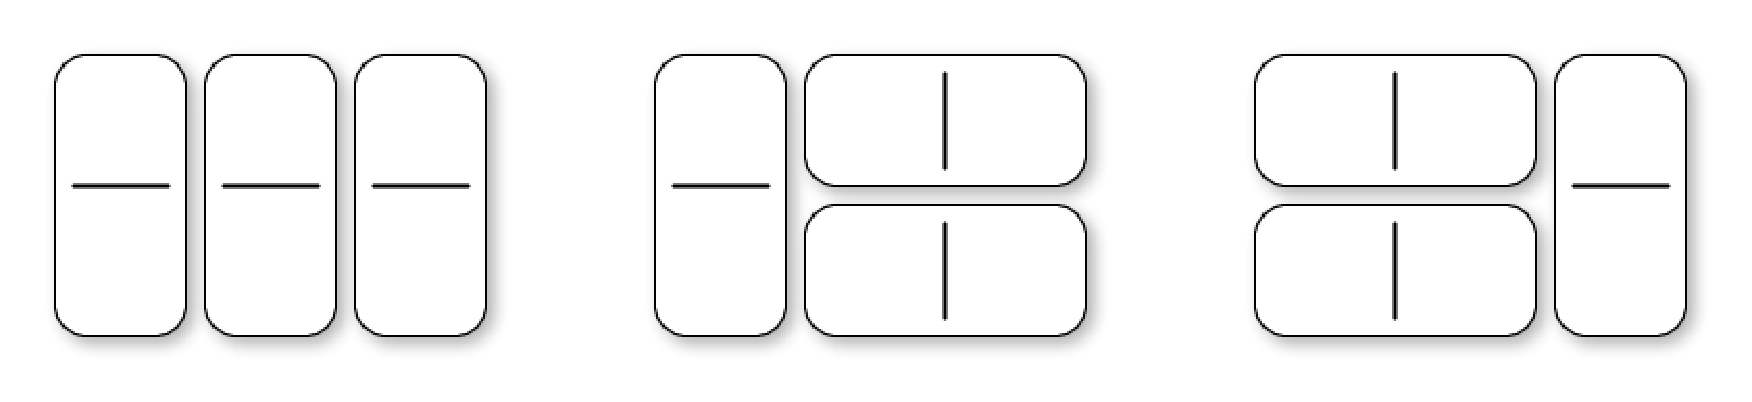
\includegraphics[width=100mm]{Figures/23-tilings.eps}
\end{center}
\vspace{-5mm}

%There is only one way to tile a $2 \times 1$ grid: 
\includegraphics[width=10mm]{Figures/21-tiling.pdf}

\noindent
(a) \mymark{1}
Draw all ways to tile a $2 \times 4$ grid.

\vfill

\noindent
(b) \mymarks{2}
Let $f(n)$ denote the number of ways to tile a $2 \times n$ grid. So $f(0) = 1, f(1) = 1, f(2) = 2$, and $f(3) = 3$.
Find $f(5)$ and $f(6)$ (you do not have to draw any tilings, 
but you can if it helps you).

\vfill
\hfill $f(5)=$ ~ ~ ~ ~

\vfill
\hfill $f(6)=$ ~ ~ ~ ~
\vfill

\noindent
(c) \mymarks{2}
Let $n \geq 2$. Assume that we know $f(k)$ 
for all values $0 \leq k \leq n-1$. 
Give a simple expression that calculates $f(n)$ 
using these known $f(k)$ values. 
Carefully justify your answer using at most {\bf two sentences}.

\vfill\vfill~

\newpage
\noindent
(d) \mymarks{2}
Write a function \texttt{tiling(n)} that returns the value $f(n)$ for a given integer $n \geq 0$. For full marks,
it should compute $f(9999)$ in less than one second.

\vfill
\vfill
\vfill

\noindent
(e) \mymark{2}
Let $g(n)$ denote the number of ways to tile a $3 \times n$ grid 
using dominoes. Here is a tiling of a $3 \times 4$ grid:

\vspace{-5mm}
\begin{center}
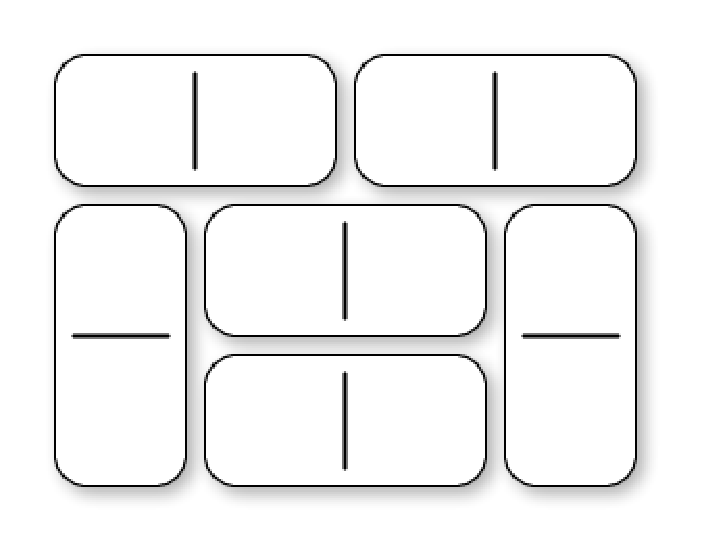
\includegraphics[width=40mm]{Figures/34-tiling.eps}
\end{center}
\vspace{-5mm}
\noindent
So, $g(0) = 1, g(2) = 3$, $g(4) = 11$, and $g(6) = 41$.

~

\noindent
What is $g(n)$ when $n$ is odd? Justify your answer.

\vfill

\noindent
(f) \mymarks{2}
Let $n \geq 2$ be an even integer. 
Assume that we know $g(k)$ for all $0 \leq k \leq n-1$. 
Give an expression that easily calculates $g(n)$
using these known $g(k)$ values. Justify your answer.


\vfill
\vfill

%=========================================================================

\newpage
\section*{question 2: ascii mazes}

One way to represent a maze using ASCII characters is
\texttt{|}-{\em format}, which uses 
vertical bars \verb&|&, underscores \verb&_&, and spaces.
A rectangular grid using only these three 
characters is a {\em valid maze} if

$\bullet$ there are at least 2 rows and at least 3 columns, and

$\bullet$ the top row has only \verb&_& characters, and

$\bullet$ the first character in the second row 
is a space, indicating the entrance, and

$\bullet$ the last character in the last row is \verb&_&,
indicating the exit, and

$\bullet$ except for the entrance and exit,
the first and last character on each row is \verb&|&,  and

$\bullet$
the bottom row has no spaces.

\noindent
\begin{minipage}[c]{3cm}
{\bf Example i}
\end{minipage}
\begin{minipage}[c]{10cm}
\begin{verbatim}
_________
  | ___ |
| | | | |
|_____|__

\end{verbatim}
\end{minipage}

In \texttt{|}-format,
a grid cell is {\em vacant} if it is a space, or
if it is not on the top row and is \verb&_&. Two vacant cells 
{\em join each other}
if one is beside the other (up, down, left, or right).
Neighbouring vacant cells join each other if 
and only if no wall separates them.

~

\noindent
(a) \mymarks{1} ~ ~
\begin{minipage}[c]{11cm}
For this maze, put a dot in each vacant cell,
and draw a line between each pair of vacant cells that 
join each other.
\end{minipage} ~ ~
\begin{minipage}[c]{3cm}
{\large\begin{verbatim}
____
  _|
| _|
|___

\end{verbatim}}
\end{minipage}

Another way to represent a maze is with \verb&X&-{\em format}.
\verb&X&-format uses a space for vacant cells and an \verb&X& otherwise.
The first character of the second row is a space,
for the entrance; 
the last character of the second-last row is a space, for the exit;
every other character on the rectangular boundary 
of this grid is \verb&X&.

\noindent
\begin{minipage}[c]{3cm}
{\bf Example ii}
\end{minipage}
\begin{minipage}[c]{10cm}
{\small\begin{verbatim}
XXXXXXXXX
  X     X
X X XXX X
X X X X X
X X X X X
X     X  
XXXXXXXXX

\end{verbatim}}
\end{minipage}

We can convert from \verb&|&-format to \verb&X&-format 
by adding extra rows, and placing a space or \verb&X&
between two cells that are on top of each other indicating 
whether they join each other.
The \verb&X&-format example above is what we get by converting from the \verb&|&-format example.
Notice that the number of vacant cells can change during this conversion.
The maze in (b) is what you would get by converting from
the maze in (a).

~

\noindent
(b) \mymarks{1} ~ ~
\begin{minipage}[c]{11cm}
For this maze, put a dot in each vacant cell,
and draw a line between each pair of vacant cells that join
each other.
\end{minipage} ~ ~
\begin{minipage}[c]{3cm}
{\small\begin{verbatim}
XXXX
   X
X XX
X  X
X XX
X  
XXXX
\end{verbatim}}
\end{minipage}

(c) \mymarks{4}
Write a function \texttt{convert(maze)} that takes an array or list of strings representing a valid maze in \verb&|&-format and 
prints the corresponding maze in \verb&X&-format. 
For example, \texttt{maze} is from (a) then
\texttt{convert(maze)} prints the maze from (b).

\vfill

(d) \mymarks{6}
Now write a function \verb&search(maze)& 
that takes an array of strings representing a maze in \verb&X&-format.
It should print a path from the entrance to the exit using 
\verb&*& characters. 
You may assume that there is exactly one way to travel from the entrance
to the exit using a path that does not visit a cell more than once.

~

\noindent
\begin{minipage}[c]{13cm}
{\bf Example}: calling \texttt{search(maze)} with \verb&X&-format 
example ii gives this output:
\end{minipage}~ ~ ~
\begin{minipage}[c]{4cm}
{\small\begin{verbatim}
XXXXXXXXX
**X*****X
X*X*XXX*X
X*X*X X*X
X*X*X X*X
X***  X**
XXXXXXXXX
\end{verbatim}}
\end{minipage}
\vfill~

%=========================================================================

\newpage
\section*{question 3: blorks}

A {\em binary string} contains only \verb&0&s and \verb&1&.
A {\em blork} is a string containing only characters \verb&0&, \verb&1&, and \verb&*&. 
A binary string \verb&str& {\em matches} a blork \verb&blrk&
if each \verb&*& character in \verb&blrk& 
can be replaced with a binary string (possibly empty, and the
binary strings do not all have to be the same)
so that the resulting string equals \verb&str&. 
We show such a matching by 
starting with the blork and then
replacing each \verb&*& with \verb&(b)& where \verb&b& is
the needed binary string for that \verb&*&.

~

\noindent
{\bf Example}
\begin{itemize}
\item \verb&str = "01001"&, \verb&blrk = "01*01"&,
{\bf match} \verb&"01(0)01"&
\item \verb&str = "101"&, \verb&blrk = "10**1"&, 
{\bf match} \verb&"10()()1"&
\item \verb&str = "10101101"&, \verb&blrk = "10*10*"&, 
{\bf match} \verb&"10(101)10(1)" and "10()10(1101)"&
\item \verb&str = ""&, \verb&blrk = ""& (both strings are empty), 
{\bf match} \verb&""&
\item \verb&str = "11101"&, \verb&blrk = "101*"&, {\bf no match possible}
\end{itemize}

~

(a) \mymarks{2}
For each of the following, indicate whether it matches. 
If yes, give one replacement, in the same form as the example.

\begin{itemize}
\item \verb&str = "1001"&, \verb&blrk = "*1*0*1*"& \\~\\
\item \verb&str = "110110001010100"&, \verb&blrk = "1101*100*10*01*"& \\~\\
\item \verb&str = "10001101001"&, \verb&blrk = "100*11*101"& \\~\\
\item \verb&str = ""&, \verb&blrk = "*"& \\~\\
\item \verb&str = "100101010100001010001011101101"&, \verb&blrk = "*1001*001*11*101"& \\~\\
\item \verb&str = "000110101101100010101010101101"&, \verb&blrk = "*1101*101010*110"& \\~\\
\end{itemize}

\newpage
(b) \mymarks{3}
Write a function \verb&extract(blrk)& that takes a blork \texttt{blrk} 
as parameter and returns an array or list of strings 
with the binary subtring {\em pieces}
of \texttt{blrk}, namely the
nonempty binary substrings left over
if each $*$ is replaced with a space.

Example: for \texttt{blrk = "*10**1110*110"} the three 
pieces are \verb&"10", "1110", "110"&.

\vfill

(c) \mymarks{5}
Write a function \verb&match(str, blrk)& that takes a binary string \verb&str& and blork \verb&blrk& as parameters and returns \verb&true& if \verb&str& matches \verb&blrk& and \verb&false& otherwise. If it is helpful, you may use the function described in part (b) even if you did not 
answer that question.

\vfill

%=========================================================================

\newpage
\section*{question 4: hex}

{\bf Warning}: this question can take time. 
Budget your time wisely.

~

The two-player game of Hex is played on an $n \times n$ 
board with hexagonal cells. Below is a $7 \times 7$ board. 
Players alternate turns. 
On a turn, a player puts a stone on an empty cell.

The first player is called {\em white} and places white stones. 
The second player is called {\em black} and places black stones. 
Two opposing sides of the board are white and the other two 
opposing sides are black.
The winner is whoever connects
their two sides with a connected path of their stones. 
In the example below, black has won.

\begin{center}

\includegraphics[width=100mm]{fz/pix/7x7-f1b6.eps}
\end{center}

An amazing property of Hex 
is that if the board is completely covered with stones then
exactly one player has joined their two sides. So draws are not possible.

~

This question is about playing perfectly in Hex.
We say that a player plays {\em perfectly} if,
on each move, if there is some move that is part
of a winning strategy for that player,
then the player makes such a move.
So, whoever can win always makes a winning move;
whoever cannot win can play anywhere.

\newpage

(a) \mymarks{3}
On this $3 \times 3$ board white played her first move 
in the middle. (The letters are for the analysis below.)
Now it is black's turn.
We claim that white can win.

\begin{center}

\includegraphics[width=40mm]{fz/pix/3x3-marked.eps}
\end{center}

White can guarantee she gets at least one of the cells labelled $x$ 
by placing a stone on one of these two cells
if black ever places a stone on the other. 
Similarly, white can guarantee she gets at least one of the cells 
labelled $y$.
But each $x$ cell touches the left side and the middle,
and each $y$ cell touches the middle and the right side.
So white will join her two sides if she follows this strategy.

~

Now assume that white starts a game by
by placing her first stone as shown below. 
It is black's turn. 
Who will win the game if both players play perfectly from now on?
Justify your answer by giving the winning player's strategy 
{\bf as concisely as possible}. 

(We have included a page with blank $3 \times 3$ hex grids
on the second last page of this exam. You can use these to help describe the strategy, just make sure that we can follow your reasoning.)

\vfill

\noindent
\hfill
\includegraphics[width=50mm]{fz/pix/3strat.eps}\
\hfill
\includegraphics[width=50mm]{fz/pix/3strat0.eps}\
\hfill
\includegraphics[width=50mm]{fz/pix/3strat1.eps}

\vfill

\noindent{\bf Solution}

(above middle)
If black's 1st move is not in the set $\{a1,a2,b1\}$ then
white wins by playing b1, and then on the next move
one of $\{a1,a2\}$. Similarly, if black's 1st move is not
in $\{a2,a3,b2\}$ then white wins by playing b2
and then on the next move one of $\{a2,a3\}$.
So white wins unless black's 1st move is in {\em both} sets, so a2.

~

(above right)
Now white wins by playing a3, and then on the next move
either b2 or (if black is already there) b3, and then 
on the next move either c2 or c3.
\vfill~

\newpage
(b) \mymarks{4}
For {\bf each} cell on the $4 \times 4$ board below, 
show who wins (white or black) if that cell is white's first move,
and both players play perfectly from then on:
if white wins, then on that cell draw an empty circle
(or the letter \texttt{W}); 
if black wins, then on that cell draw a filled circle 
(or the letter \texttt{B}).

You do not need to justify your answer:
your score will be calculated as follows:
\[ \max\left\{\frac{({\rm \#~of~correct~answers}) - ({\rm \#~of~incorrect~answers})}{4}, \:\:\:\: 0\right\}. \]
Cells left blank will be counted neither correct nor incorrect.
Illegible entries will be counted incorrect.
(Some empty $4 \times 4$ grids can be found at the end of this exam. These are for your scratch notes only and will not be looked at when we grade.)

~

\noindent{\bf Solution}

\begin{center}

\includegraphics[width=60mm]{fz/pix/4x4.winners.eps}\
\end{center}

~

White wins by playing b3, as shown (below left).
By a symmetric strategy (reflect the board through the 
centermost point) white also wins by playing c2.
So far we have two winning openings.

~


\includegraphics[width=60mm]{fz/pix/4.1strat2.eps}\

\includegraphics[width=60mm]{fz/pix/4x4.winners0.eps}

~

\newpage
If white plays first in any of the unmarked cells
below left, then black can win. By also considering the 
symmetric black strategy, we now have 10 losing openings (below right).

~


\includegraphics[width=60mm]{fz/pix/4.1strat.eps}\

\includegraphics[width=60mm]{fz/pix/4x4.winners1.eps}

~

White can win by playing first at a4.
If black's reply is not in \{b3,b4,c3,d2,d3\}
then white wins by next playing c3.
If black's reply is in one of these 5 cells,
then white wins by playing c2.
This is easy to see if black played in \{b3,c3,d3\},
and not too hard to see if black played in \{b4,d2\}.
One such line of play is shown below.

By symmetry, White also wins by playing first at d1.


\includegraphics[width=60mm]{fz/pix/4z.eps}

\includegraphics[width=60mm]{fz/pix/4x4.winners2.eps}
~

There are only two opening moves left, and they are symmetric.
If white plays first at c1 (below left), black can win:
the main variation is shown, this is not a complete proof.
By symmetry, if white plays first at b4, black wins.
So we are done.

~


\includegraphics[width=60mm]{fz/pix/4last.eps}\

\includegraphics[width=60mm]{fz/pix/4x4.winners.eps}

~

PS. Ryan Hayward is writing a book on Hex. If you would like
to be notified when it is published, send him email:
\verb+hayward@ualberta.ca+ .

%=========================================================================

\newpage
\begin{center}

\includegraphics[width=40mm]{fz/pix/3x3.eps}~~~~~~
\includegraphics[width=40mm]{fz/pix/3x3.eps}~~~~~~
\includegraphics[width=40mm]{fz/pix/3x3.eps}\vfill

\includegraphics[width=40mm]{fz/pix/3x3.eps}~~~~~~
\includegraphics[width=40mm]{fz/pix/3x3.eps}~~~~~~
\includegraphics[width=40mm]{fz/pix/3x3.eps}\vfill

\includegraphics[width=40mm]{fz/pix/3x3.eps}~~~~~~
\includegraphics[width=40mm]{fz/pix/3x3.eps}~~~~~~
\includegraphics[width=40mm]{fz/pix/3x3.eps}\vfill

\includegraphics[width=40mm]{fz/pix/3x3.eps}~~~~~~
\includegraphics[width=40mm]{fz/pix/3x3.eps}~~~~~~
\includegraphics[width=40mm]{fz/pix/3x3.eps}\vfill

\includegraphics[width=40mm]{fz/pix/3x3.eps}~~~~~~
\includegraphics[width=40mm]{fz/pix/3x3.eps}~~~~~~
\includegraphics[width=40mm]{fz/pix/3x3.eps}
\end{center}

%=========================================================================

\newpage
\begin{center}
{\bf this page will not be graded}

\includegraphics[width=40mm]{fz/pix/4x4.eps}~~~~~~
\includegraphics[width=40mm]{fz/pix/4x4.eps}~~~~~~
\includegraphics[width=40mm]{fz/pix/4x4.eps}\vfill

\includegraphics[width=40mm]{fz/pix/4x4.eps}~~~~~~
\includegraphics[width=40mm]{fz/pix/4x4.eps}~~~~~~
\includegraphics[width=40mm]{fz/pix/4x4.eps}\vfill

\includegraphics[width=40mm]{fz/pix/4x4.eps}~~~~~~
\includegraphics[width=40mm]{fz/pix/4x4.eps}~~~~~~
\includegraphics[width=40mm]{fz/pix/4x4.eps}\vfill

\includegraphics[width=40mm]{fz/pix/4x4.eps}~~~~~~
\includegraphics[width=40mm]{fz/pix/4x4.eps}~~~~~~
\includegraphics[width=40mm]{fz/pix/4x4.eps}\vfill

\includegraphics[width=40mm]{fz/pix/4x4.eps}~~~~~~
\includegraphics[width=40mm]{fz/pix/4x4.eps}~~~~~~
\includegraphics[width=40mm]{fz/pix/4x4.eps}\vfill

\includegraphics[width=40mm]{fz/pix/4x4.eps}~~~~~~
\includegraphics[width=40mm]{fz/pix/4x4.eps}~~~~~~
\includegraphics[width=40mm]{fz/pix/4x4.eps}
\end{center}


%=========================================================================
\end{document}
